% MA211 - Lecture 20
\documentclass[pdftex, xcolor=pdftex, dvipsnames,handout]{beamer}

\usetheme{MA211}
\usepackage{thumbpdf}
\usepackage{wasysym}
%\usepackage{ucs}
\usepackage[utf8]{inputenc}
\usepackage{pgf,pgfarrows,pgfnodes,pgfautomata,pgfheaps,pgfshade}
\usepackage{verbatim}

\usepackage{eurosym}
\usepackage{euler}

\usepackage{calc}               % Simple computations with LaTeX variables
%\usepackage[hang]{caption2}     % Improved captions

\usepackage{graphicx}           % Standard graphics package

\usepackage{amsmath, amsthm, amssymb}


\newcommand{\fquad}{\mbox{\qquad}}
\newcommand{\bull}{$\bullet$ }

\newcommand {\I} {\mathcal I}
\newcommand {\calI} {\mathcal I}
\def\disint{\displaystyle\int}

\DeclareMathOperator{\D}{d}
\newcommand{\dydx}{\frac{\D y}{\D x}}

%\definecolor{gray}{rgb}{0.69, 0.69, 0.69} \newcommand{\gray}[1]{\textcolor{gray}{#1}}
\definecolor{dogreen}{rgb}{0.33, 0.42, 0.18} \newcommand{\dogreen}[1]{\textcolor{dogreen}{#1}}
\definecolor{maroon}{rgb}{.5,0.2,0.2}\newcommand{\maroon}[1]{\textcolor{maroon}{#1}}
\definecolor{greena}{rgb}{.1,0.581,0.1}\newcommand{\greena}[1]{\textcolor{greena}{#1}}

\definecolor{blue4}{rgb}{0,0,.545}
\newcommand{\Blue}[1]{\textcolor{blue}{#1}}
\newcommand{\Red}[1]{\textcolor{red}{#1}}
\definecolor{pink}{rgb}{1.,0.75,0.8}
\definecolor{darkred}{rgb}{0.5,0.0,0.0}
\definecolor{darkgreen}{rgb}{0,0.3,0.3}
\definecolor{purple}{rgb}{0,0.3,0.3}
\definecolor{darkblue}{rgb}{0.0, 0.0, .5}
\definecolor{dpurple}{rgb}{.3,.0,.3}
\newcommand{\Green}[1]{\textcolor{darkgreen}{#1}}
\newcommand{\DRed}[1]{\textcolor{darkred}{#1}}
\newcommand{\DBlue}[1]{\textcolor{darkblue}{#1}}
\newcommand{\Purple}[1]{\textcolor{dpurple}{#1}}
\newcommand{\Emph}[1]{\textcolor{darkred}{\textbf{\it #1}}}
\newcommand{\remph}[1]{\textcolor{darkred}{\textbf{\emph{#1}}}}
\newcommand{\bemph}[1]{\textcolor{darkblue}{\textbf{\emph{#1}}}}
\newcommand{\gemph}[1]{\textcolor{darkgreen}{\textbf{\emph{#1}}}}
\newcommand{\Bf}[1]{\textcolor{darkblue}{\textbf{#1}}}
\newcommand{\Gf}[1]{\textcolor{darkgreen}{\textbf{#1}}}
\newcommand{\Rf}[1]{\textcolor{red}{\textbf{#1}}}
\newcommand{\Rmf}[1]{\textcolor{red}{\mathbf{#1}}}

\newcommand{\Conj}[1]{\overline{#1}}

\newcommand{\code}[1]{\textcolor{darkblue}{\texttt{\textbf{#1}}}}
\newcommand{\icode}[1]{{\blue\texttt{\textbf{\emph{#1}}}}}
\newcommand{\gcode}[1]{{\Green{\texttt{\textbf{\emph{#1}}}}}}
\newcommand{\out}[1]{\texttt{\emph{\textbf{\Green{#1}}}}}





\newenvironment{vminipage}%
{\begin{Sbox}\begin{minipage}\begin{small}\begin{verbatim}}%
{\end{verbatim}\end{small}\end{minipage}\end{Sbox}\fbox{\TheSbox}}

\newenvironment{nminipage}%
{\begin{Sbox}\begin{minipage}}%
{\end{minipage}\end{Sbox}\fbox{\TheSbox}}


\let\Arg\relax\DeclareMathOperator{\Arg}{\mathtt{Arg}}
\let\Arg\relax\DeclareMathOperator{\e}{\mathtt{e}}

\newcommand {\AND} {\wedge}
\newcommand {\OR} {\vee}
\newcommand {\NOT} {\neg}
\newcommand {\IMPLIES} {\rightarrow}
%\newcommand {\IFF} {\leftrightarrow}
\renewcommand {\iff} {\Leftrightarrow}
\newcommand {\NAND} {\uparrow}
\newcommand {\NOR} {\downarrow}
\newcommand {\XOR} {\otimes}

\newenvironment{citemize}% Colour items
{\begin{description}}%
{\end{description}}

\newcommand {\maroonitem}{\item[\maroon{$\bullet$}]}

\newcommand {\gitem} {\item {\includegraphics[width=.4cm,angle=-10]{img/green-bullet-on-white.ps}}}
\newcommand {\ritem} {\item {\includegraphics[width=.4cm,angle=-10]{img/red-bullet-on-white.ps}}}
\newcommand {\yitem} {\item {\includegraphics[width=.4cm,angle=-10]{img/yellow-bullet-on-white.ps}}}
\newcommand {\bitem} {\item {\includegraphics[width=.4cm,angle=-10]{img/blue-bullet-on-white.ps}}}

\newcommand {\greenitem} {\item {\includegraphics[width=.4cm,angle=-10]{img/green-bullet-on-white.ps}}}
\newcommand {\reditem} {\item {\includegraphics[width=.4cm,angle=-10]{img/red-bullet-on-white.ps}}}
\newcommand {\yellowitem} {\item {\includegraphics[width=.4cm,angle=-10]{img/yellow-bullet-on-white.ps}}}
\newcommand {\blueitem} {\item {\includegraphics[width=.4cm,angle=-10]{img/blue-bullet-on-white.ps}}}

\newcommand {\eq}[1]%
  {$\DBlue{#1}$}
\newcommand {\eqd}[1]%
  {$\displaystyle\DBlue{#1}$}
%\newcommand{\eq}[1]{\boldmath \DBlue{$#1$}}


\newcommand {\csf}{\centerslidesfalse}
\newcommand {\cst}{\centerslidestrue}

\newcommand {\vecii}[2] {   \big(\begin{smallmatrix} #1 \\ #2 \end{smallmatrix}\big)}
\newcommand{\atwo}[2]{\left(\!\!\begin{array}{c} #1 \\ #2 \end{array}\!\!\right)}


\newcommand{\C}{\mathbb{C}}
\newcommand{\Q}{\mathbb{Q}}
\newcommand{\R}{\mathbb{R}}
\newcommand{\N}{\mathbb{N}}
\newcommand{\Z}{\protect\mathbb{Z}}  % protect for index.
\newcommand {\Rs}{ \mathbb{R}}
\newcommand {\Cs}{ \mathbb{C}}
\newcommand {\Rnn}{ \mathbb{R}^{n \times n}}
\newcommand {\Rn}{ \mathbb{R}^{n}}


\newcommand{\mblock}{%
\setbeamercolor*{block title}{bg=maroon,fg=white}
\setbeamercolor*{block body}{bg=white,fg=maroon}
}%

\newcommand{\bblock}{%
\setbeamercolor*{block title}{bg=Steel,fg=white}
\setbeamercolor*{block body}{bg=Mylightgray,fg=Steel}
}%

\newcommand{\gblock}{%
\setbeamercolor*{block title}{bg=Green,fg=white}
\setbeamercolor*{block body}{bg=Mylightgray,fg=darkgreen}
}%


\newcommand{\rblock}{%
\setbeamercolor*{block title}{bg=Red,fg=white}
\setbeamercolor*{block body}{bg=white,fg=Black}
}%

\def\disfrac{\displaystyle\frac}
\newcommand{\TakeNotes}{
\includegraphics[width=2cm]{TakeNote}}

\def\eps{\varepsilon}
\newcommand {\del}[2]{ {\frac{\partial #1}{\partial #2}}}
\newcommand {\x}[1]{x^{[#1]}}
\newcommand {\delx}{ {\frac{\partial}{\partial x}}}
\newcommand {\delt}{ {\frac{\partial}{\partial t}}}
\newcommand {\dely}{ {\frac{\partial}{\partial y}}}
\newcommand {\ith}{{(i)}}
\renewcommand {\vec}[1]{ {\boldsymbol{#1}}}
\newcommand {\Oh} {\mathcal O}
\newcommand {\Err} {\mathcal E}
%\newcommand {\th} {\mathrm{th}}
\DeclareMathOperator{\fl}{fl}
\DeclareMathOperator{\sign}{sign}
\DeclareMathOperator{\Cond}{Cond} 
\DeclareMathOperator{\cond}{cond}
\DeclareMathOperator{\diag}{diag} 
\DeclareMathOperator{\sym}{sym} 
\DeclareMathOperator{\Trace}{Trace}

\DeclareMathOperator{\E}{e}

\newcommand {\Rsym}{{ \mathbb{R}^{n \times n}_\mathrm{sym}}}

\newcommand {\st} {\mathrm{st}}
\newcommand {\nd} {\mathrm{nd}}


\parskip .25cm


\theoremstyle{definition}
\newtheorem{exercise}{Exercise}[section]
\newtheorem{method}{Method}[section]

\newcommand{\Header}[1]{\begin{center}{\Large \Bf{#1}}\end{center}}

\subtitle{MA211}
\title{Lecture 20: Improper Integrals -- Type 2}

\author{Dr Niall Madden}

\date{\Large Monday $17^\mathrm{th}$ Nov 2008}


\begin{document}

\setcounter{framenumber}{-1}
\frame{

%\begin{columns}[c]
%\column{0.45\textwidth}
%\centering
%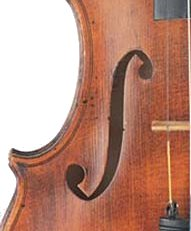
\includegraphics[width=4cm]{images/violin}
%
%
%\column{0.55\textwidth}
\begin{block}{}
\begin{center}
\begin{large}
 \insertsubtitle
\end{large}

\vspace{.1cm}

\begin{Large}
\textbf{\inserttitle}
\end{Large}


\vspace{.3cm}

{\insertdate}

\end{center}
\end{block}

\begin{center}
%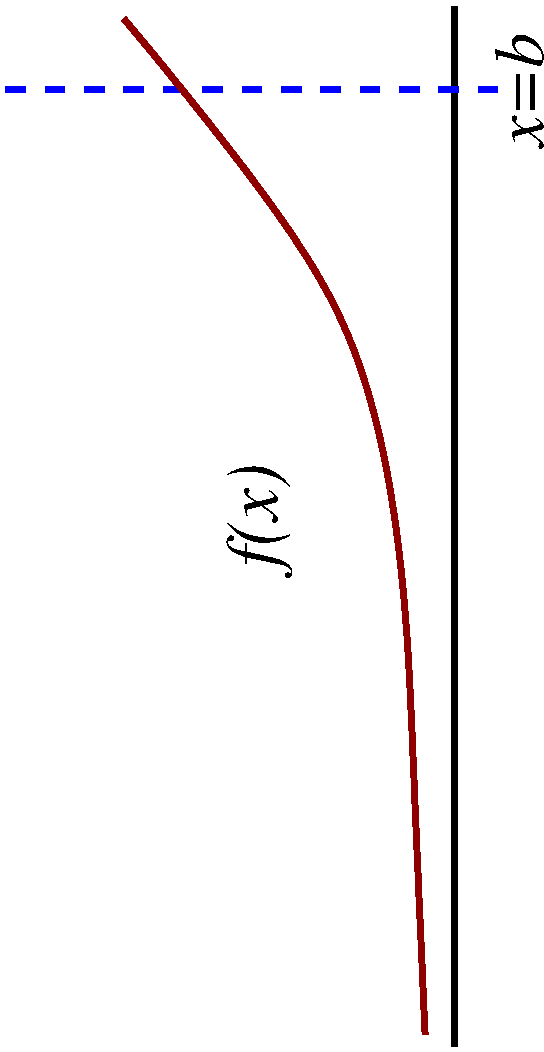
\includegraphics[width=2.4cm,angle=-90]{images/Improper1a}
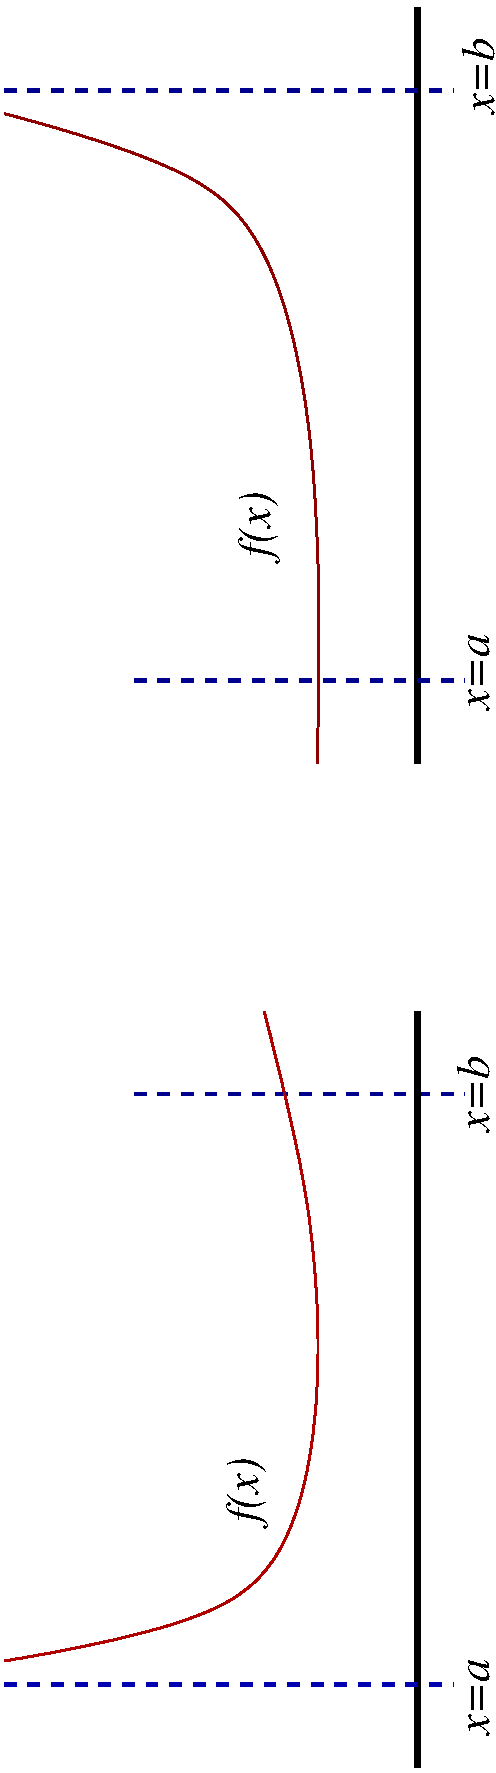
\includegraphics[width=3cm,angle=-90]{images/Improper2}
\end{center}


% \end{columns}

}

\frame{
  \frametitle{Topics of the day...}

%\begin{columns}[c]
%\column{0.5\textwidth}
 \tableofcontents
%\column{0.5\textwidth}


See also Section 7.7 of Stewart.

%\end{columns}
}




\section{Improper Integrals: Type 2}
\frame{

Last week we saw how to evaluate improper integrals of \Emph{Type 1}
where the limits of integration include one or both of \eq{-\infty} or
\eq{\infty}, e.g.,

\begin{block}{Improper Integrals: Type 1}

\[\int_{-\infty}^b f(x) dx, ~~ \quad
\int_{a}^\infty f(x) dx, ~~ \quad
\int_{-\infty}^\infty f(x) dx\]
\end{block}

How we'll look at Improper Integrals \Emph{of Type 2}
\[ 
\int_{a}^b f(x) dx,\quad
\text{ where } f(x) \rightarrow \pm \infty\] at \eq{a}, \eq{b} or somewhere in
between.
 
}

\frame{

In particular, we want to evaluate 
\[ \int_{a}^{b} f(x)\,dx \] where \eq{f(x)} may be unbounded at \eq{a}
or \eq{b}, or at some point in between.
\vspace{-1cm}
\begin{center}
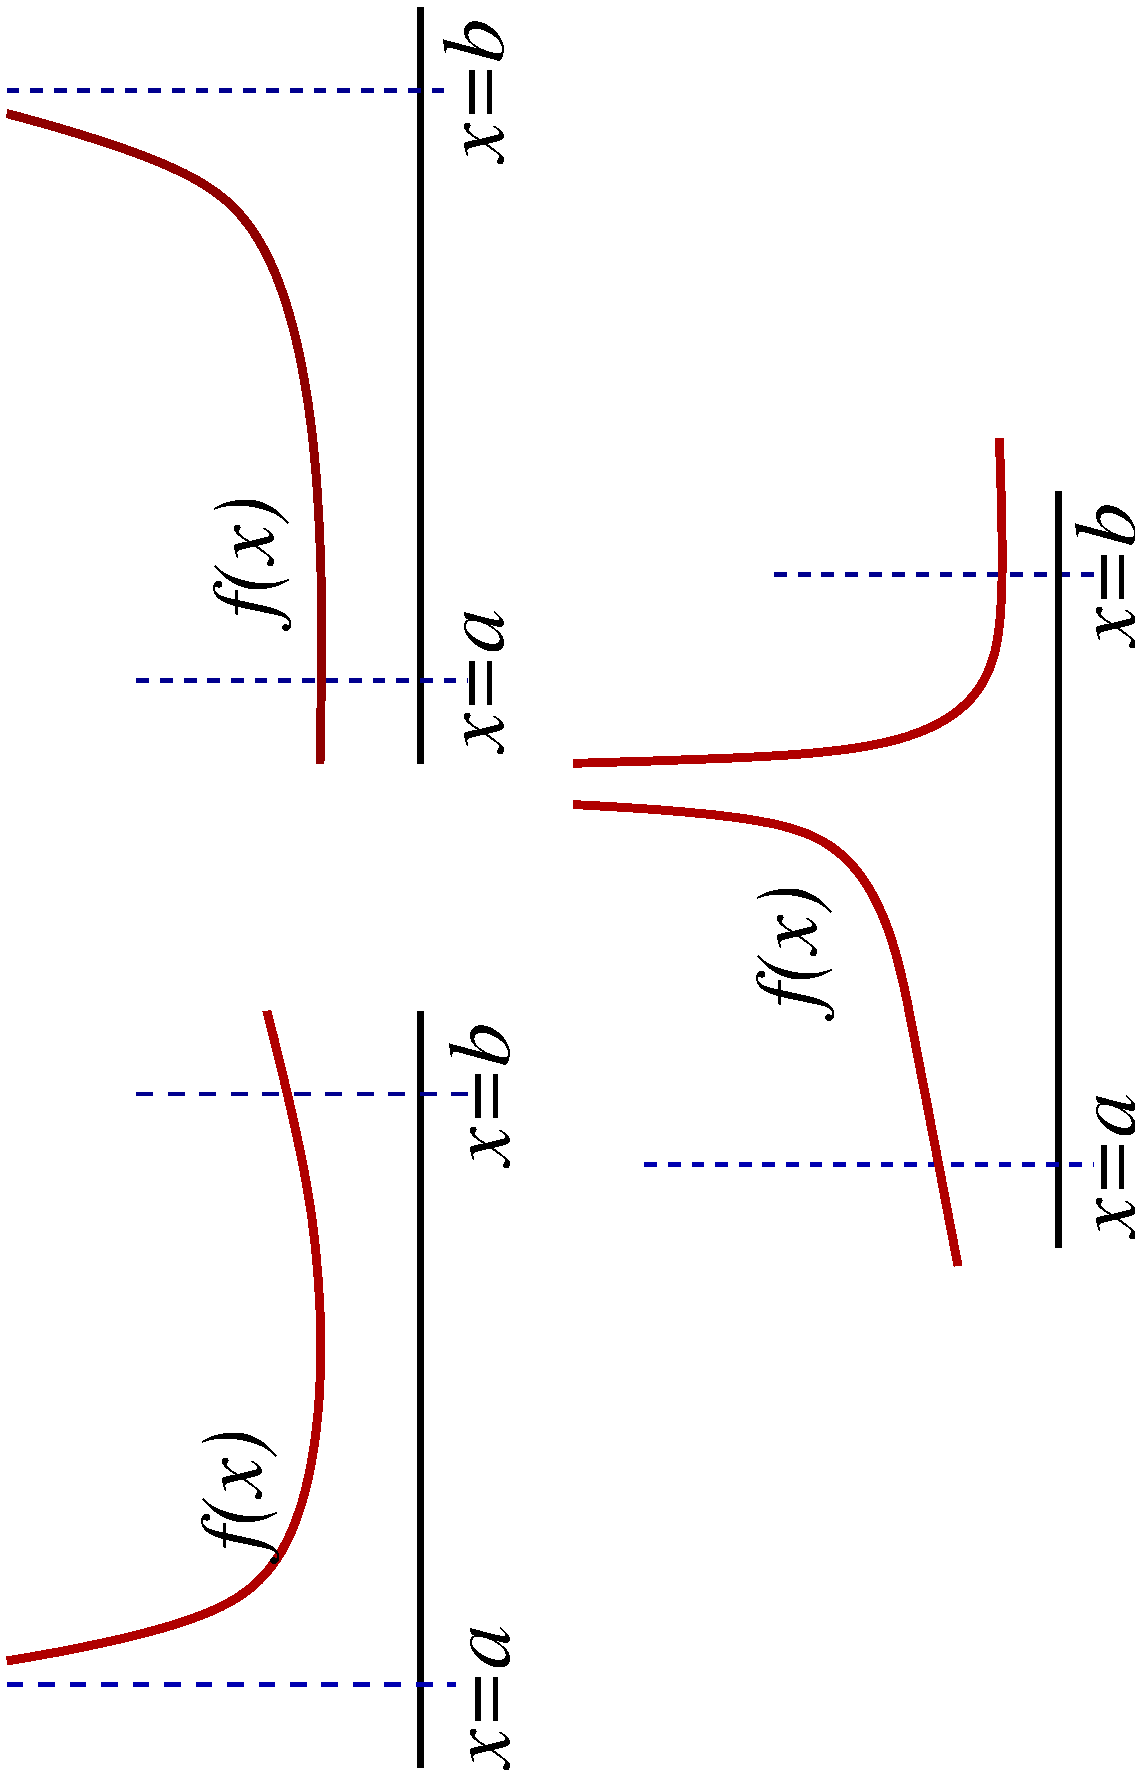
\includegraphics[angle=-90,width=8cm]{images/Improper2A}
\end{center}

}

\frame{

\Header{\eq{f(x)} unbounded at $x=a$}

When function \eq{f(x)} is defined for \eq{a < x \leq b} then 
evaluate \eqd{\I(t) = \int_t^b f(x) dx} and then use that:
\[
\int_a^b f(x) dx =  \lim_{t \to a^+} \int_t^b f(x) dx.
\]
So:
\vspace{-0.4cm}
\begin{enumerate}[<+->]
\item Evaluate \eqd{\I(t) = \int_t^b f(x) dx}
\item Compute the limit  \eqd{L=  \lim_{t \to a^+} \I(t)}
\item If \eq{L} is finite then \eqd{\int_{a}^{b} f(x)\,dx = L}, and we
  can say that \eq{\int_{a}^{b} f(x)\,dx} \textbf{converges to $L$}. 

\item If \eq{L} is \Emph{not} finite, then  integral is said to
diverge.
\end{enumerate}

}

\frame{
\begin{example}
Does the integral $\displaystyle\int_{0}^{1} \frac{1}{x}dx$ converge?
\end{example}

\vspace{4cm}

}


\frame{
\begin{example}
Evaluate the improper integral $\displaystyle\int_{0}^{1}
\frac{1}{x^2}dx$ 
\end{example} \vspace{3.4cm}
}


\frame{
\begin{example}
Evaluate the TYPE 2 Improper Integral $\displaystyle\int_{0}^{1}
\frac{1}{\sqrt{x}}dx$ 
\end{example} \vspace{3.4cm}

}



\frame{
\begin{small}
\begin{block}{}%{The general case}
\eqd{\int_{0}^{1} x^{-p}dx} will  \Emph{converge}
when  $p < 1$,  and \Bf{diverge} for $p\geq 1$.
\end{block}
\Bf{Proof:}
\pause
If  $p=1$ then
\eqd{ ~  \int_t^1 x^{-p} dx = \int_t^1 \frac{1}{x} dx =
  \ln(x)\bigg|_t^1 = \ln(t) - \ln(1) = \ln(t).}\\
But \eqd{\lim_{t\to 0} \ln(t)} does not exists,  so \eqd{\int_0^1 \frac{1}{x} dx}
diverges. \pause

If $p \neq 1$  then \eqd{\int_t^1 x^{-p}dx = \frac{x^{1-p}}{1-p}\bigg|_t^1 =
    \frac{1 - t^{1-p}}{1-p}}. \\ \pause
If $p<1$ then $1-p>\alert{0}$ so the limit \eqd{\lim_{t \to 0}  t^{1-p}=0}.
So the integral converges to  \eqd{\frac{1}{1-p}}.\\ \pause
If however $p>1$ then $1-p<\alert{0}$ and  \eqd{\lim_{t \to 0}  t^{1-p}} does
not exist, so the integral \Bf{diverges}.
\end{small}
}

%\frame{
%\begin{example}
%Does the  $\displaystyle\int_{0}^{1} \frac{\ln(x)}{x}dx$ converge
%or diverge?
%\end{example}
%\vspace{4cm}
%}

\frame{
If \eqd{f}  is defined on \eq{[a,b)} and \eqd{\lim_{t \rightarrow
b^-} \int_{a}^{t} f(x)\,dx} exists, call the limit  \eq{L} and write
\[ 
\int_{a}^{b} f(x)\,dx = L.
\]

Again, $\int_{a}^{b} f(x)\,dx$ is said to {\bf converge to $L$}. If no
such limit exists, the integral is divergent.
}
\frame{
\begin{example}
Does the  $\displaystyle\int_{0}^{4} \frac{dx}{\sqrt{4-x}}$ converge
or diverge?
\end{example}
\vspace{4cm}
}




\frame{

If a function $f$ is defined on $[a,b]$ except at some point $c$
in $(a,b)$ at which $f$ is \Emph{unbounded}, then use that
\[ \int_{a}^{b} f(x)\,dx = \int_{a}^{c} f(x)\,dx + \int_{c}^{b}
f(x)\,dx.
\]

The integral  converges if and only if  \eqd{\int_{a}^{c}
  f(x)\,dx}  and \eqd{\int_{c}^{b} f(x)\,dx} \Bf{both} converge.

\begin{example}
Does the improper integral \eqd{\displaystyle\int_{-1}^{1}
  \frac{dx}{x}}
 converge or diverge?
\end{example}

}


\section{The Comparison Test}


\frame{
Earlier we saw how to evaluate \eqd{ \int_{1}^{\infty}
  \frac{1}{1+x^2}{dx}}.

But suppose we just wanted to determine if it 
\alert{converges} or \alert{diverges}...

\vspace{4cm}
}

\frame{

Often, we just want to know if some integral converges or diverges --
and not necessarily evaluate the integral.

In that case we can compare the integral with one that we know.
This is helpful because we  can use the \Emph{Comparison Test}...

}



\frame{
\begin{block}{Comparison Test}
Suppose $f$ and $g$ are defined on $[a, \infty)$ and 
\[ 0 \leq f(x) \leq g(x) \text{ for all }  x \in [a, \infty).\]
 Then
\[ \int_a^\infty  f(x) dx \leq \int_a^\infty g(x) dx.\]
Therefore
\begin{enumerate}
\item If $\int_{a}^{\infty} g(x)\,dx$ \Bf{converges}, so does
$\int_{a}^{\infty} f(x)\,dx$  
\item if $\int_{a}^{\infty} f(x)\,dx$ \Emph{diverges}, so does $\int_{a}^{\infty} g(x)\,dx$
 \end{enumerate}
\end{block}

  There are corresponding results for the other types of improper
  integrals.
}

\frame{
\begin{example}
Does the integral \eqd{\displaystyle\int_{1}^{\infty} \frac{dx}{
    x^2 + x^3}} converge or diverge?
\end{example}

\vspace{3cm}
}


%\frame{
%\begin{example}
%  $\displaystyle\int_{1}^{\infty}\frac{dx}{ x + x^2}$ 
%\end{example}
%
%\vspace{3cm}
%}




\frame{
\rblock
\begin{example}
Does the improper integral  $\displaystyle\int_{0}^{1}\frac{dx}{ 2x^2
  + 3x^3}$
converge or diverge?
\end{example}

\vspace{4cm}
}

\frame{
\begin{example}
Establish if  $\displaystyle\int_{0}^{1}\frac{dx}{ 2\sqrt{x} + x^2}$
is convergent or divergent.
\end{example}

\alert{NOTE: The solution given to this one in class was wrong.}

\Bf{Correct answer:} For \eq{0 \leq x \leq 1} we know that $\sqrt{x} \geq
x^2$, so 
\[ 2\sqrt{x} + x^2 \geq 3 \sqrt{x}.\]
Thus
\[
\frac{1}{ 2\sqrt{x} + x^2} \leq \frac{1}{3}\frac{1}{\sqrt{x}} \leq
  \frac{1}{\sqrt{x}}.
\]

But we know that \eqd{\int_0^1 x^{-1/2} dx} converges, so by the
Comparison Principal, so too does 
\eqd{\int_{0}^{1}\frac{dx}{ 2\sqrt{x} + x^2}}.

}

\frame{
\begin{example}
Test for convergence of the following integral:
\[ 
  \int_{1}^{\infty}\frac{\cos x\,dx}{ 1 + x^2}
\]
\end{example}

}



\frame{

\begin{exercise}[Q20.1]
 For each of the following integrals, determine if they
  \emph{converge} or \emph{diverge}
\begin{enumerate}[(i)]
\item  \eqd{\int_1^{\infty} \frac{|\cos(x)|}{x^3+2}dx}.
\hfill (ii)~\eqd{\int_0^{1} \frac{dx}{x^{5/3}}dx}.
\item[(iii)]  \eqd{\int_0^{1} \frac{dx}{x^{3/5}}dx}.
\hfill (iv)  \eqd{\int_0^{\infty} \frac{x}{x^{3/2} + 2x^2}dx}.
\item[(v)]  ~\eqd{\int_{-2}^2 \frac{1}{\mathbf{{x}^2}} dx}
\hfill (vi) \eqd{\int_{1}^\infty \frac{1}{\sqrt{x+x^4}} dx}
\end{enumerate}
\end{exercise}
}



\end{document}

\section{Recall: 1st Order Differential Equations}
\frame{

At the beginning of the course, we looked briefly at 1st Order Differential
Equations.

Later we  studied some  2nd order problems with constant
coefficients.

Now we return to 1st Order problems with non-constant coefficients.
These can't be solved with the simple substitution \eq{y=e^{rx}}:
we'll need to use the Techniques of Integration that we learnt over
that last 2 weeks.

}

\frame{

\begin{block}{}
As \Emph{1st Order Differential Equation} is of the form
\begin{center}
\eqd{\frac{dy}{dx} = f(x,y)}.
\end{center}
That is: the right hand side is some function of both \eq{x} and \eq{y}.

\pause
\Emph{Solving} the equation means expressing the relationship between
\eq{x} and \eq{y} in a manner not involving derivatives. 
\end{block}
\pause
The approaches that we will study are
\begin{enumerate}[<+->]
\item Separable DEs (today)
\item Homogeneous DEs 
\item Integrating Factors.
\end{enumerate}
}


%\section{Separable and Homogeneous 1st Order Equations}
\section{Recall: Separable  Equations}
\frame{


\begin{block}{}
A first order equation \eqd{\frac{dy}{dx} = f(x, y)} is \Bf{separable}
if we can write \eq{f(x)} as the product of some functions $g(x)$ and
$h(y)$. That is, it has the form 
\[
\frac{dy}{dx} =g(x)h(y).
\]
\pause
Such an equation can be solved by writing 
\[
\frac{1}{h(y)}dy = g(x)\,dx
\]
and integrating both sides:
\[
\int \frac{1}{h(y)}dy = \int g(x)\,dx
\]
\end{block}
}



\frame{
\begin{example}
Solve the equation \eqd{\alert{\frac{dy}{dx}}=e^{x-y}}.
\end{example}

\vspace{4cm}
%\noindent\und{Solution}: We have $\disfrac{dy}{dx}=\disfrac{e^x}{e^y}$.
%Thus $e^y\,dy = e^x dx$, and 
%$$
%\int e^y\,dy = \int e^x\,dx \Longrightarrow e^y =- e^x + C.
%$$
%Thus solutions are given by $y(x)=\ln (e^x+C)$, for a constant $C$.

}

\frame{
\begin{exercise}
Find the general solution to the 1st order separable DEs
\begin{enumerate}
\item \eqd{\frac{dy}{dx}= \frac{x}{y}}. 
\item \eqd{\frac{dy}{dx}= \frac{y}{x}}. 
\end{enumerate}
\end{exercise}
}



\frame{
\begin{example}
Solve $\disfrac{dy}{dx}=\sqrt{y}\cos^2\big(\sqrt{y}\big)$.
\end{example}

\vspace{4.5cm}

%\noindent\und{Solution}: We have $\disfrac{1}{\sqrt{y}\cos^2\sqrt{y}}\,dy =
%dx$. Thus 
%$$
%\int\frac{1}{\sqrt{y}\cos^2\sqrt{y}}\,dy = \int\,dx.
%$$
%Let $u=\sqrt{y}$. Then $\disfrac{du}{dy}=\disfrac{1}{2}y^{-1/2}$ and
%$\disfrac{1}{\sqrt{y}}\,dy = 2\,du$. Thus 
%$$
%2\int \sec^2 u\,du = \int\,dx \Longrightarrow 2\tan u = x+C.
%$$
%Solution : $2\tan(\sqrt{y}) = x+C$.
}

\frame{
\begin{exercise}
Solve the differential equation
\[
\frac{dy}{dx} = y \ln(x).
\]
\end{exercise}
}


\frame{
\begin{example}
Solve the equation $\disfrac{dy}{dx} = \frac{xy-2y+x-2}{x+3}$. 
\end{example}
\pause
\Bf{Solution}: This equation is separable : 
\[
\frac{dy}{dx} = \frac{(x-2)(y+1)}{x+3}\Longrightarrow
\frac{dy}{y+1}=\frac{x-2}{x+3}\,dx.
\]
Then...
\vspace{3.4cm}
%$$
%\int\frac{dy}{y+1} = \int\frac{x-2}{x+3}\,dx =
%\int\frac{x}{x+3}\,dx-2\int\frac{1}{x+3}\,dx. 
%$$
%If $u=x+3$ then $x=u-3$, $dx=du$ and 
%$$
%\int\frac{x}{x+3} = \int 1-\frac{3}{u}\,du = u - 3\ln |u| (+c).
%$$
%Now integrating gives 
%$$
%\ln |y+1| = x+3-3\ln |x+3|-2\ln |x+3| +C = x+3-5\ln |x+3| +C.
%$$

}

\frame{
\begin{example}[MA211, Semester 1 2006, Q3 (d)]
Solve the differential equation
\[
\frac{dy}{dx} = -(y^2 + 2y +2)(x+1)\ln(x) \text{ with }
y(1)=-1
\]
\end{example}
\vspace{2cm}

}

\frame{
\begin{exercise}
Find the general solution to the following differential equations:
\begin{enumerate}
\begin{columns}[c]
\column{3cm}
\item \eqd{  \frac{dy}{dx} = \disfrac{y}{2x}.}
\item \eqd{  \frac{dy}{dx} = \disfrac{e^x}{\sin(y)}.}
\column{3cm}
\item \eqd{  \frac{dy}{dx} = e^y{\sin(x)}.}
\item \eqd{  \frac{dy}{dx} = {y}{\ln(x)}.}
\end{columns}

\end{enumerate}
\end{exercise}

\begin{exercise}
Solve the following initial value problems:
\begin{enumerate}
\item \eqd{  \frac{dy}{dx} = 3 + e^y; \quad y(0)=1.}
\item \eqd{  \frac{dy}{dx} = \sinh(x)e^{-y} \quad y(0)=1};
\end{enumerate}
\end{exercise}

}

\section{Homogeneous Equations}
\frame{


The first order differential equation \eqd{\frac{dy}{dx}=f(x,y)} is
called \Emph{homogeneous} if \eqd{f(x,y)} can be written as a function of
\eqd{\frac{y}{x}}, i.e. 
$$
\disfrac{dy}{dx} = h\left(\frac{y}{x}\right).
$$
\pause
In this situation if we write \eqd{v = \disfrac{y}{x}}, we have
\eqd{y=vx}. 
\pause
Differentiate to get:
\[
\frac{dy}{dx} = v + x\disfrac{dv}{dx}.\]
\pause 
Substitute into the original differential equation:
\[ v + x\disfrac{dv}{dx} = h(v).\]
\pause
This equation involving $v$ and $x$ is separable:
\[ \frac{1}{h(v)-v}dv=\frac{1}{x}dx\]
}

\frame{

\begin{example}
Solve the equation $\disfrac{dy}{dx}=\disfrac{xy+y^2}{x^2}$.
\end{example}
%
%\n\und{Solution}: $\disfrac{dy}{dx} =
%\disfrac{y}{x}+\left(\disfrac{y}{x}\right)^2$, so the equation is
%homogeneous. \\
%Write $v = \disfrac{y}{x}$. Then $\disfrac{dy}{dx} = v +
%x\disfrac{dv}{dx}$ and 
%$$
%v + x\disfrac{dv}{dx} = v+v^2\Longrightarrow x\disfrac{dv}{dx} = v^2.
%$$
%Thus 
%$$
%\frac{1}{v^2}\,dv = \frac{1}{x}\,dx\Longrightarrow
%\int\frac{1}{v^2}\,dv = \int\frac{1}{x}\,dx.
%$$
%Hence 
%$$
%-\frac{1}{v} = \ln |x|+C\Longrightarrow v = \frac{y}{x} =
%\frac{-1}{\ln |x|+C}.
%$$
%Solution : $y = \disfrac{-x}{\ln |x|+C}$. 

\vspace{4cm}
}


\frame{
\begin{example}
Solve the following initial value problem:
\[ 
  \frac{dy}{dx} = \disfrac{x^2 + xy}{xy + y^2}, \qquad y(2)=1.
\]
\end{example}
\vspace{4cm}
}

\frame{
\begin{exercise}
Find the general solution to the following differential equations:
\begin{enumerate}
\item \eqd{  \frac{dy}{dx} = \disfrac{x + y}{x - y}.}
\item \eqd{  \frac{dy}{dx} = \disfrac{xy}{x^2 +2y^2}.}
\end{enumerate}
\end{exercise}

\begin{exercise}
Solve the following initial value problems:
\begin{enumerate}
\item \eqd{  \frac{dy}{dx} = \disfrac{x^2 + xy + y^2}{x^2}; \quad y(1)=1.}
\item \eqd{  \frac{dy}{dx} = \disfrac{x^3 + 3xy^2}{3x^2y + y^3};
    \qquad y(1)=-1}
\end{enumerate}
\end{exercise}

}


\end{document}

